\begin{figure}[htbp]
    \centering
    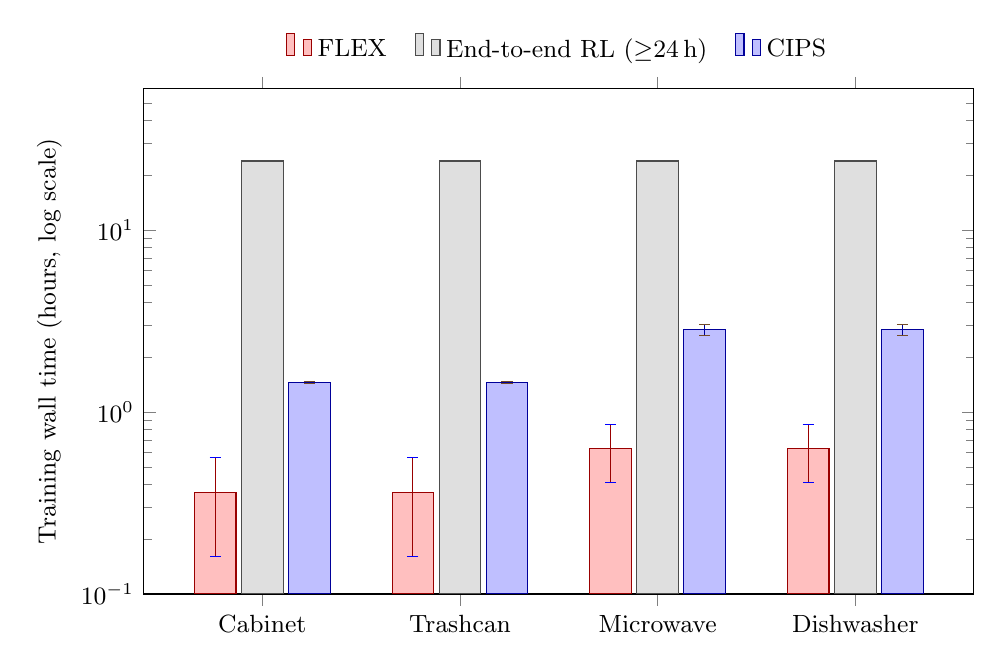
\begin{tikzpicture}
    \begin{axis}[
        ybar=2pt,
        bar width=15pt,
        width=\textwidth, height=8cm,
        enlarge x limits=0.2,
        ymode=log,
        log origin=infty,
        ymin=0.1, ymax=60,
        ylabel={Training wall time (hours, log scale)},
        symbolic x coords={Cabinet, Trashcan, Microwave, Dishwasher},
        xtick={Cabinet, Trashcan, Microwave, Dishwasher},
        legend style={at={(0.5,1.03)}, anchor=south, legend columns=3,
                      font=\small, draw=none, /tikz/every even column/.append style={column sep=8pt}},
        error bars/y dir=both, error bars/y explicit,
        tick label style={font=\small},
        label style={font=\small},
    ]
    % FLEX
    \addplot+[draw=red!60!black, fill=red!25] coordinates {
        (Cabinet,0.36) +- (0,0.2) (Trashcan,0.36) +- (0,0.2)
        (Microwave,0.63) +- (0,0.22) (Dishwasher,0.63) +- (0,0.22) };
    % End-to-end RL (>= 24 hours)
    \addplot+[draw=gray!60!black, fill=gray!25] coordinates {
        (Cabinet,24) (Trashcan,24) (Microwave,24) (Dishwasher,24) };
    % CIPS
    \addplot+[draw=blue!60!black, fill=blue!25] coordinates {
        (Cabinet,1.46) +- (0,0.02) (Trashcan,1.46) +- (0,0.02)
        (Microwave,2.84) +- (0,0.2) (Dishwasher,2.84) +- (0,0.2) };
    \legend{FLEX, End-to-end RL ($\geq$24\,h), CIPS}
    \end{axis}
    \end{tikzpicture}
    \caption{Bar-chart visualization of the training wall time reported in \cref{tab:flex_results} (log scale, lower is better). Error bars denote one standard deviation; GAMMA is omitted as it is a pre-trained perception model with no training cost reported. FLEX trains one to two orders of magnitude faster than the reinforcement learning baselines, with end-to-end RL requiring at least $24$ hours to reach even negligible success.}
    \label{fig:flex_walltime_bars}
\end{figure}
